\documentclass{beamer}
\usepackage{animate}
\usepackage{xcolor}
\usepackage{tcolorbox}
\usepackage{colortbl}
\usepackage{tikz}
\usepackage{subfig}
\usepackage{graphicx}
\usepackage{tabularx}
\usepackage{tablefootnote}
\usepackage{stackengine}% for put note about source below image
\usepackage{hyperref}
\usepackage[font=footnotesize,labelfont=bf]{caption}
\hypersetup{pdfpagemode={UseOutlines},
bookmarksopen=true,
bookmarksopenlevel=0,
hypertexnames=false,
% different link colours
colorlinks=true,% Set to false to disable coloring links
citecolor=imperial_navy,% The color of citations
linkcolor=imperial_light_blue,% The color of references to document elements (sections, figures, etc) (including contents page)
urlcolor=imperial_blue,% The color of hyperlinks (URLs)
pdfstartview={FitV},
unicode,
breaklinks=true,
}

\usepackage[backend = bibtex, style = authoryear, natbib = true]{biblatex} % Use the bibtex backend with the authoryear

% \addbibresource{mybib.bib} % The filename of the bibliography



\usetheme[sectionpage=none, progressbar=frametitle]{metropolis}
\captionsetup[figure]{justification=centering, singlelinecheck=false, font=tiny,
  format=hang}
\captionsetup[subfigure]{justification=centering, font=tiny,labelfont={bf,sf}}

\makeatletter
\setlength{\metropolis@titleseparator@linewidth}{1.5pt}
\setlength{\metropolis@progressonsectionpage@linewidth}{1.5pt}
\setlength{\metropolis@progressinheadfoot@linewidth}{1.5pt}
\makeatother


\setbeamercolor{separation line}{use=structure,bg=tangerine}
\setbeamercolor{background canvas}{bg=white}
\setbeamercolor{palette primary}{fg=white, bg=imperial_blue}

\definecolor{maroon}{RGB}{180,0,0}
\definecolor{sacramento}{RGB}{0, 85, 35} % edited
\definecolor{darkSacramento}{RGB}{0, 70, 35} % edited
\definecolor{burntOrange}{RGB}{204,85,0}
\definecolor{lightgray2}{RGB}{220,220,220} % edited
\definecolor{grey_green}{RGB}{198,203,171}
\definecolor{gen_green}{RGB}{0,128,0}
\definecolor{emerald}{RGB}{4, 99, 7}
\definecolor{forest}{RGB}{12, 102,35}

% Define imperial colours
\definecolor{imperial_navy}{RGB}{0,33,71}
\definecolor{imperial_blue}{RGB}{0,62,116}
\definecolor{imperial_light_blue}{RGB}{212,239,252}
\definecolor{imperial_normal_blue}{RGB}{0,110,175}
\definecolor{imperial_dark_teal}{RGB}{15,130,145}
\definecolor{grey_blue}{RGB}{178, 198, 221}
\definecolor{tangerine}{RGB}{236, 115, 0}

\setbeamercolor{frametitle}{bg=imperial_blue}
\setbeamercolor{section in head/foot}{bg=imperial_blue, fg= white}
\setbeamercolor{progress bar in head/foot}{bg=lightgray, fg=tangerine}
\setbeamercolor{progress bar}{bg=lightgray, fg=tangerine}
\setbeamercolor{title separator}{fg=tangerine, bg=tangerine}

\setbeamertemplate{headline}{%
  \begin{beamercolorbox}[ht=2.50ex,dp=3.50ex]{section in head/foot}
  \insertnavigation{\paperwidth} % navigation circles
  \end{beamercolorbox}%
  \begin{beamercolorbox}[colsep=0.3pt]{lower separation line head}
  \end{beamercolorbox}

 % Subsection
 %\begin{beamercolorbox}[ht=2.125ex,dp=1.125ex,%
 % leftskip=.3cm,rightskip=.3cm plus1fil]{subsection in head/foot}
 % \usebeamerfont{subsection in head/foot}\insertsubsectionhead
 % \end{beamercolorbox}%
}



% --------------------------------------------------- %
%                  Presentation info	              %
% --------------------------------------------------- %
\title{ J-IDEA Away Day}
\subtitle{Creating a Tweet-based proxy for adherence to protective behaviour}
\author{Tristan Naidoo}
\institute{}
\date{12 October 2022}

\subject{} % metadata

% --------------------------------------------------- %
%                    Title + Schedule                 %
% --------------------------------------------------- %

\begin{document}
\begin{frame}[plain, noframenumbering]
\tikz [remember picture,overlay]
    \node at
        ([xshift=-4cm, yshift=8.5cm]current page.south) 
        {
\includegraphics[height=.1\textheight]{figures/imperial.pdf}};
 \tikz [remember picture,overlay]
    \node at
        ([xshift=4.65cm, yshift=8.5cm]current page.south) 
        {
\includegraphics[height=.15\textheight]{figures/jameel_institute.png}};
 \tikz [remember picture,overlay]
    \node at
        ([xshift=1.6cm, yshift=2cm]current page.south) 
        {
\includegraphics[height=.2\textheight]{figures/twitter_logo.png}};
 \tikz [remember picture,overlay]
    \node at
        ([xshift=4.2cm, yshift=2cm]current page.south) 
        {
\includegraphics[height=.25\textheight]{figures/virus_blue.png}};
 \titlepage
\end{frame}

% --------------------------------------------------- %
%                      Presentation                   %
% --------------------------------------------------- % 
\section{Background}
\begin{frame}{PhD topic}
  \begin{itemize}
  \item No examples in the literature of analysing the relationship between
    Tweets and COVID-19 endpoints \\[10pt]
  \item Goal: Create a metric for adherence to protective behaviour over the
    COVID-19 pandemic \\[10pt]
  \item Objectives:
   \begin{enumerate}
   \item Quantify Twitter usage, sentiment, and disinformation \\[5pt]
   \item Assess the relationship between the Tweet variables and COVID-19
     outcomes of interest
   \end{enumerate}
  \end{itemize}

 
\end{frame}

\section{Data}
\begin{frame}{Quantifying Twitter usage}
\begin{itemize}
 \item  Data is gathered \href{https://developer.twitter.com/en/products/twitter-api/academic-research}{Twitter academic
    API} \\[5pt]
 \item  The API allows you search for individual search terms
\end{itemize}
\begin{figure}[!ht]
  \centering
  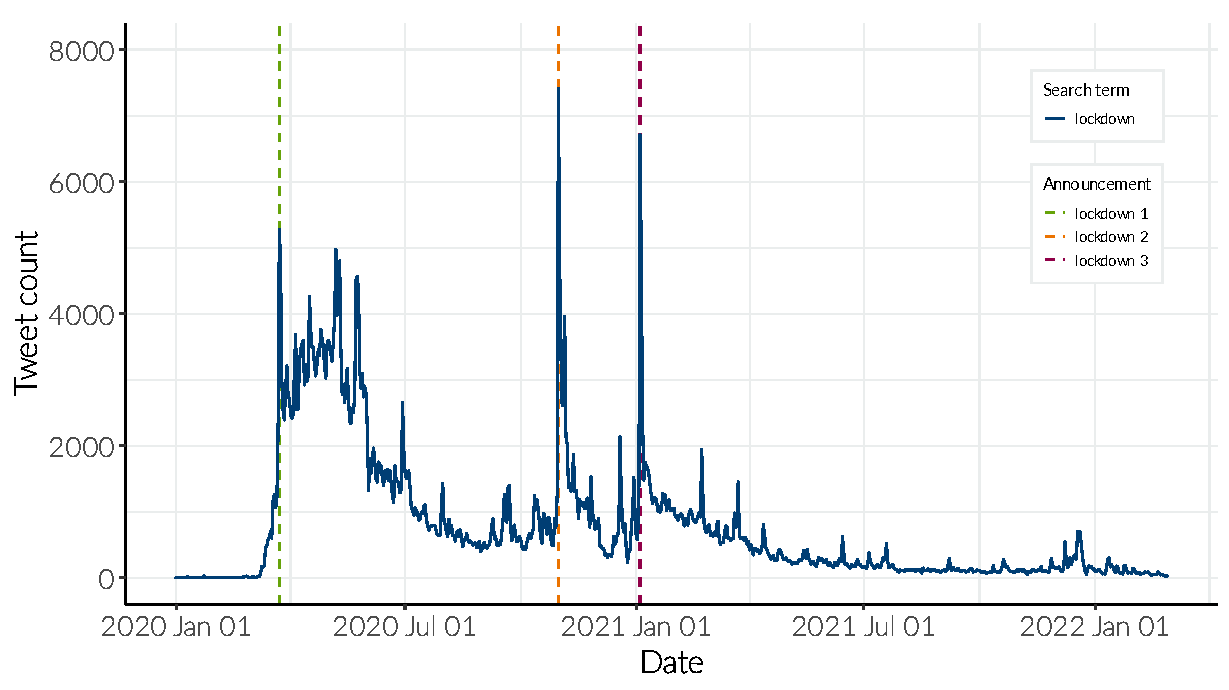
\includegraphics[width=0.8\textwidth]{figures/lockdown_count.pdf}
  \caption{Count time series using the search term \texttt{lockdown} with
    lockdown announcements superimposed}
\end{figure} 
\end{frame}

\begin{frame}{Tweet usage over time}
  \begin{itemize}
  \item Initially there is a rapid increase in the count of tweets\\[5pt]
  \item Spikes correspond to events
  \end{itemize}

  \begin{figure}[!ht]
    \centering
    \animategraphics[autoplay,
    width=\textwidth]{4}{figures/barchart_gif/barchart_}{1}{104}
    \caption{Bar chart of top 5 search terms per category over time}
  \end{figure} 
\end{frame}


\begin{frame}{Tweet usage over time}
  \begin{itemize}
  \item Three categories (number of search terms): \\ Covid-19 (25) | Policy
    (47) | Vaccine (21) \\[5pt]
  \item The number of Tweets has declined over time
  \end{itemize}
  \begin{figure}[!ht]
    \centering
    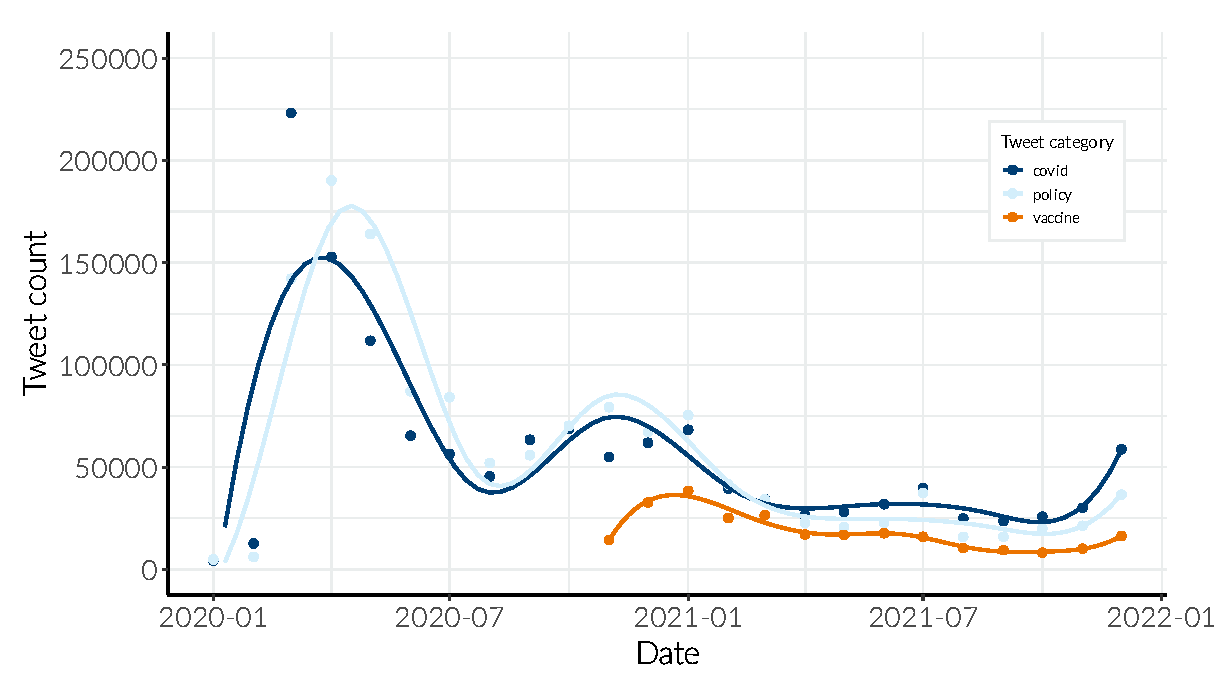
\includegraphics[width=0.8\textwidth]{figures/smoothing_spline_trend.pdf}
    \caption{Monthly Tweet counts with a smoothing spline superimposed per category}
  \end{figure} 
\end{frame}

\begin{frame}{Correlation matrix} 
  \begin{itemize}
  \item Max absolute correlation over 14 lags
  \item Correlations $>$ 0.5 for the Tweet variables highlighted
  \end{itemize}
 
  \begin{figure}[!ht]
    \centering
    \includegraphics<1>[width=0.9\textwidth]{figures/rrs_heatmap_formatted_wave2.pdf}%
    \includegraphics<2>[width=0.9\textwidth]{figures/rrs_heatmap_formatted_wave2_recs.pdf} 
    \caption{Heatmap of Spearman correlations (key below)\\PT: Policy Tweets | CT: Covid Tweets | VT: Vaccine Tweets | d: deaths | c: cases | h: hospitalisations}
  \end{figure} 
\end{frame}

 \begin{frame}{Correlation matrix} 
  \begin{itemize}
  \item Max absolute correlation over 14 lags
  \item Correlations $>$ 0.5 for the Tweet variables highlighted
  \end{itemize}
  
  \begin{figure}[!ht]
    \centering
    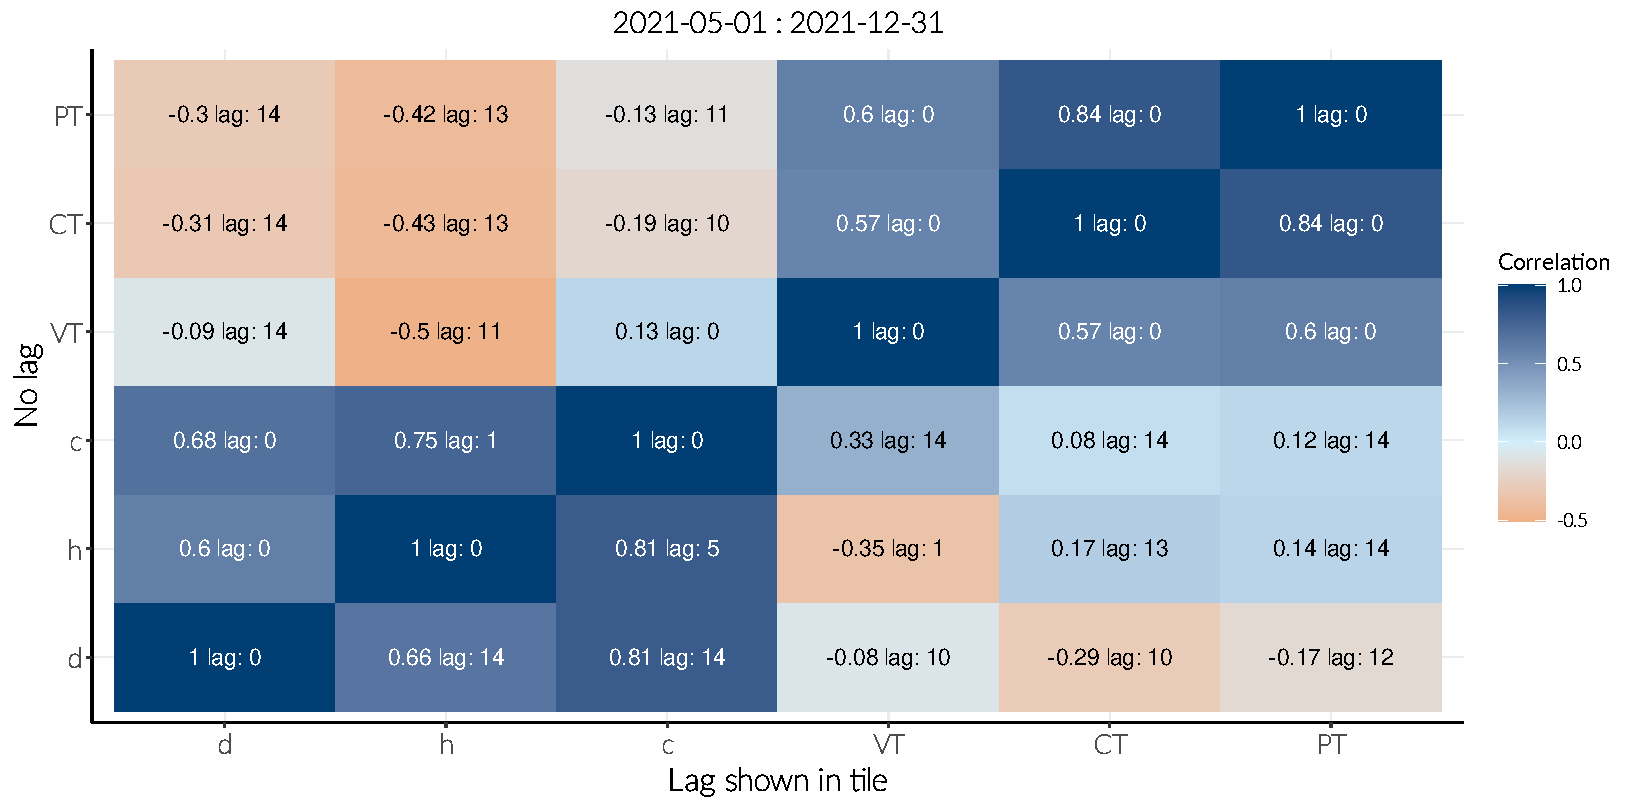
\includegraphics[width=0.9\textwidth]{figures/rrs_heatmap_formatted_wave3.pdf}
    \caption{Heatmap of Spearman correlations (key below)\\PT: Policy Tweets | CT: Covid Tweets | VT: Vaccine Tweets | d: deaths | c: cases | h: hospitalisations}
  \end{figure} 
\end{frame}


\section{Experiment}
\begin{frame}{Experiment setup}
  \begin{itemize}
  \item How informative is Tweet usage? \\[10pt]
  \item Experiment: Can Tweets improve an AR model \\[10pt]
  \item Variables: \\[5pt]
    Response | cases, hospitalisations, and deaths \\[5pt]  
    Tweet \hspace{0.5cm}| covid, policy, and vaccine \\[5pt] 
    Control \hspace{0.125cm}  | population vaccine efficacy and active variant
  \end{itemize}
\end{frame}

\begin{frame}{Modelling framework}
  \begin{itemize}
  \item 80:20 train, test split (5 consecutive day pieces) \\[5pt]
  \item Lag hyper-parameter determined by leave-one-out cross-validation 
  \end{itemize}
 \begin{figure}[!ht]
    \centering
    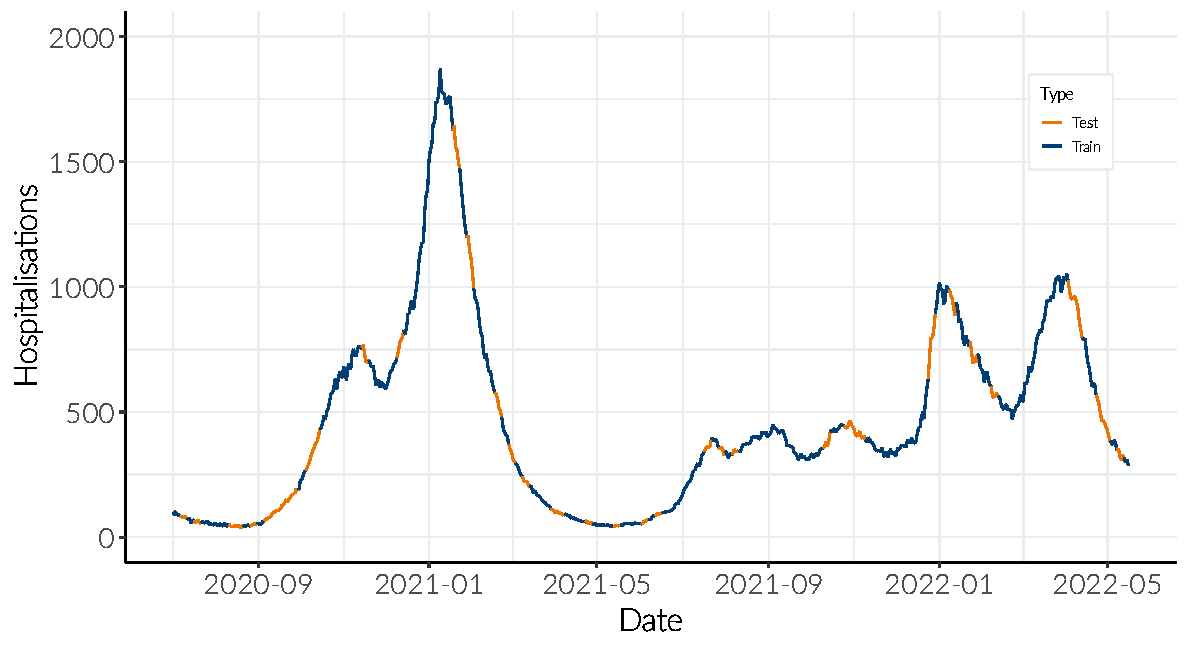
\includegraphics[width=0.8\textwidth]{figures/train_test_split.pdf} 
    \caption{Example of a train-test split across Hospitalisations}
  \end{figure}
\end{frame}

\begin{frame}{Initial results}
  \begin{itemize}
   \item Tried the experiment using Poisson GLM and log responses\\[3pt]
   \item Log response models have lower RMSE \\[3pt]
   \item Tweet variables did not improve the AR model
   \end{itemize}
  
  \begin{figure}[!ht]
    \centering
    \includegraphics<1>[width=0.8\textwidth]{figures/result_plot_full.pdf}% 
    \includegraphics<2>[width=0.8\textwidth]{figures/result_plot_train_p.pdf}% 
    \includegraphics<3>[width=0.8\textwidth]{figures/result_plot_test_p.pdf}%
    \caption{Predicted versus actual Hospitalisations; predictions are
      made using an AR(12) | Tweet(1) model  }
  \end{figure}
\end{frame}


\section{Future work}
\begin{frame}{Next steps}
  \begin{itemize}
    \item Extract raw Tweet
    \begin{itemize}
    \item Geotagging and extracting demographic information is a challenge \\[10pt]
    \end{itemize}
  \item Extend the current analysis to include sentiment and disinformation \\[10pt] 
  \item Extend analysis to other countries
  \end{itemize}
\end{frame}

\end{document}


